\section{Versuchsdurchführung}
\label{sec:durchfuerung}

\subsection{Einstellen der Temperaturprofile}
\subsubsection*{Vorbereitung des Thermostates und des Reaktors}
Begonnen wurde die Versuchsdurchführung durch Inbetriebnahme des Thermostats. Hierfür wurden die Gewebe-PVC-Schläuche über einen Schlauch-Gewinde-Adapter mit dem 2L-Reaktor verbunden. Das jeweils andere Ende der Schläuche war bereits mit dem Thermostat über Schlauchschellen befestigt. Für die Verbindung mit dem Thermostat war es zu beachten, dass der Schlauch mit dem heizenden Vorlaufstrom an der unteren Seite des Reaktors festgeschraubt wurde, Luftblasen im Reaktormantel zu vermeiden. Danach wurden ebenfalls über Schlauchschellen weitere PVC-Schläuche mit den Ein- und Ausgänge der Thermostatkühlung verbunden. Der eingehende Schlauch wurde auf der anderen Seite mit einem Wasseranschluss (ungeöffnet) versehen. Der ausgehende Schlauch führte in einen Ausguss. Nun konnte das Thermostat eingeschaltet werden und es meldete sich sofort eine Fehlermeldung E01, welche in diesem Fall auf einen zu niedrigen Füllstand im Behälter des Thermostates hinwies. Nach Auffüllen des Theromstatbades wurde das Gerät erneut ohne Fehlermeldung gestartet und nun war es dem Thermostat manuell eine Solltemperatur zu geben und den Prozess zu starten. Um jedoch mit Temperaturrampen arbeiten zu können, war das Herstellen einer Verbindung zu einem PC mit der \textsc{Julabo Easy Temp} Software nötig.
\subsubsection*{Konfigurieren des Thermostates}
Hierfür wurde der Computer und das Thermostat mittels Kabel über die verfügbaren RS-232-Schnittellen miteinander verbunden. Durch gleichzeitiges Drücken der Cursortaste \keys{\arrowkeyleft} und der Entertaste \keys{\return} gelangte man in die Konfigurationsebene des Thermostates und konnte die in Tabelle \ref{tab:thermostat_config} aufgeführten Einstellungen für die Fernsteuerung mittels Computer einstellen. Über die Tasten \keys{\arrowkeyleft} und \keys{\arrowkeyright} ließ sich nun der gewünschte Parameter auswählen und über die Tasten \keys{\arrowkeyup} und  \keys{\arrowkeydown} dessen Wert verändern. Jede Änderung musste mit der Entertaste \keys{\return} bestätigt werden. Durch erneut gleichzeitiges Drücken der Cursortaste \keys{\arrowkeyleft} und der Entertaste \keys{\return} wurde die Konfigurationsebene des Thermostats wieder verlassen. Auf dem Display der Thermostates war nun die Meldung \texttt{rOFF} zu sehen.
\subsubsection*{Konfigurieren des Computers}
Nachdem das Thermostat konfiguriert wurde, erfolgte eine weitere Konfiguration am PC mit der \textsc{Julabo Easy Temp} Software. Nach dem Starten des Programms wurde zu \menu{Geräte>Geräte konfigurieren} navigiert und es öffnete sich ein Fenster. Unter \menu{Gerät hinzufügen} können nun die Einstellungen aus Tabelle \ref{tab:thermostat_config} für den Computer konfiguriert werden.
\begin{table}[h!]
	\renewcommand*{\arraystretch}{1.2}
	\centering
	\caption{Konfigurationen \textsc{Julabo} Thermostat MW und \textsc{Easy Temp}-Software}
	\label{tab:thermostat_config}
	\begin{tabulary}{1.0\textwidth}{C|C|C}
		\hline
		\textbf{Gerät} & \textbf{Parameter} & \textbf{Wert}\\
		\hline
		\multirow{5}{*}{Thermostat} & \texttt{Atc} & \texttt{0}\\
		& \texttt{H} & \texttt{1}\\
		& \texttt{P} & \texttt{2}\\
		& \texttt{Br} & \texttt{48}\\
		& \texttt{r} & \texttt{1}\\
		\hline
		\multirow{3}{*}{Software} & \texttt{Gerät} & \texttt{TopTechMXs}\\
		& \texttt{Anschluss} & \texttt{COM 1}\\
		& \texttt{Bautenrate} & \texttt{48000 s}\\
		\hline			
	\end{tabulary}
\end{table}%
\FloatBarrier

Als dies erfolgt war, konnten alle Einstellungen übernommen werden und es öffnet sich ein Fenster wie in Abbildung \ref{fig:fenster_standby_online}. Über das Feld \texttt{Online} wurde bestätigt, dass eine Verbindung mit dem Thermostat hergestellt wurde. Über einen Klick auf das graue Feld \texttt{Standby} konnte das Thermostat nun gestartet werden und das Feld wechselte die Farbe auf grün und zeigte das Wort \texttt{Start} an. Das Thermostat regelte die Temperatur des Heizfluides (hier: Wasser) nun auf die angegebene Solltemperatur (hier: 80°C). Über einen Klick auf die Solltemperatur, ließ sich dieser Wert auch ändern.

\begin{figure}[h!]
	\centering
	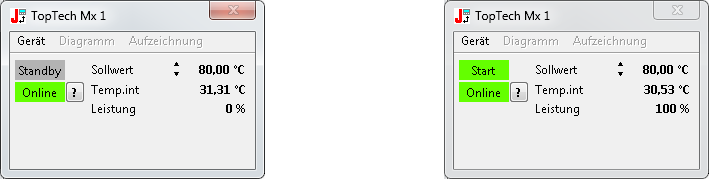
\includegraphics[width=1.0\textwidth]{img/julabo_2}
	\caption{Gerätefenster der \textsc{Easy Temp} Software zum starten des Thermostates}
	\label{fig:fenster_standby_online}
\end{figure}
\FloatBarrier
%Ende

\subsubsection*{Kurvendarstellung am PC - \textsc{Easy Temp} Software}
Nachdem nun das Thermostat und der PC miteinander kommunizieren konnten, bestand nun auch die Möglichkeit sich den Temperaturverlauf des Heißfluides darstellen zu lassen. Hierfür navigierte man im Hauptfenster des Programms nach \menu{Ansicht>Kurven bearbeiten} und es öffnete sich das Fenster der Kurvenkonfiguration, welches in Abb. \ref{fig:kurvenkonfig} zu sehen ist. Über die Schaltfläche \menu{Hinzufügen} konnte nun ein neues Gerät hinzugefügt werden, sowie der darzustellende Messwert ausgewählt und Namen für den Messwert vergeben werden. In diesem Versuch wurden der Sollwert und die interne Temperatur im Thermostat ausgewählt und infolge dieser Einstellungen geplottet (vgl. Abb. \ref{fig:beispiel_plot}).

\begin{figure}[h!]
	\centering
	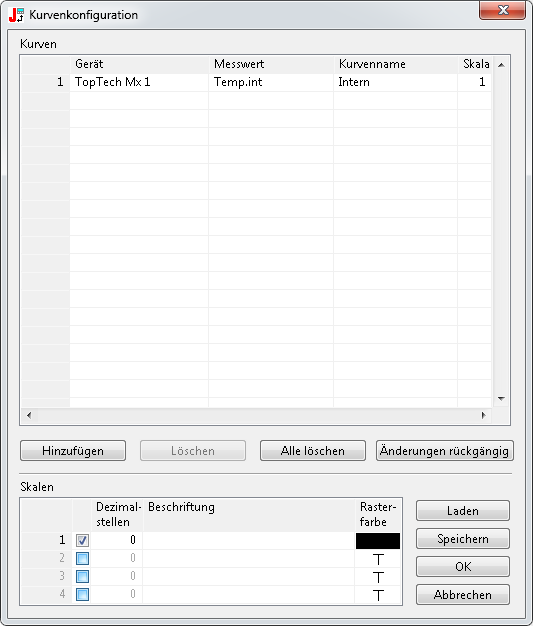
\includegraphics[width=0.5\textwidth]{img/julabo_3}
	\caption{Kurvenkonfiguration der \textsc{Easy Temp} Software}
	\label{fig:kurvenkonfig}
\end{figure}
\FloatBarrier
%Ende

\begin{figure}[h!]
	\centering
	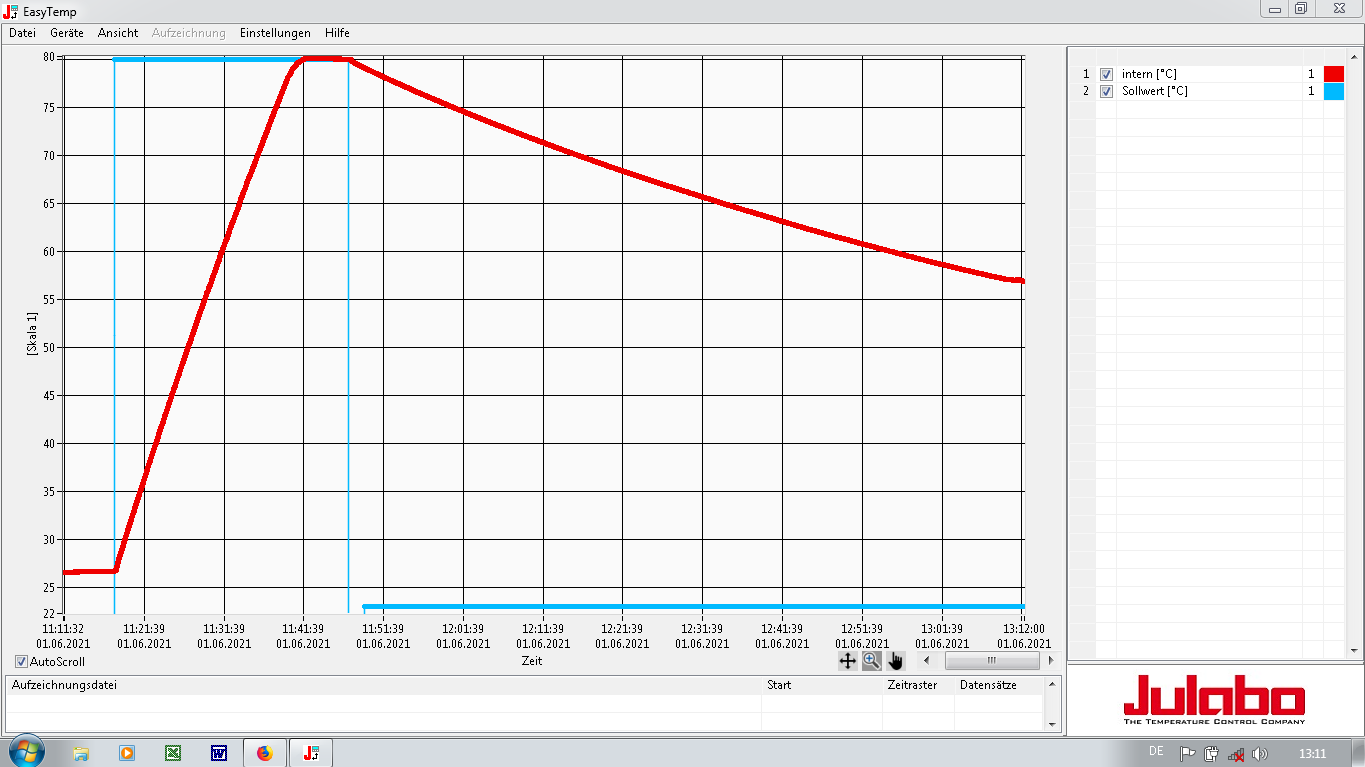
\includegraphics[width=0.75\textwidth]{img/julabo_4}
	\caption{Beispiel einer Messwertaufnahme in \textsc{Easy Temp}}
	\label{fig:beispiel_plot}
\end{figure}
\FloatBarrier
%Ende

\subsubsection*{Zeitmessung der Heiz- und Abkühlvorgänge}
Für eine grobe Abschätzung der Dauer der geforderten Prozesse wurden das Aufheizen des leeren Reaktor beginnend bei \SI{25}{\celsius} und das Abkühlen von zuvor einzustellenden \SI{80}{\celsius} wieder auf \SI{25}{\celsius} gemessen. Die \SI{25}{\celsius} werden hierbei als Raumtemperatur angenommen. Diese Abschätzungen sollten in der weiteren Versuchsdurchführung dazu dienen, die Temperaturprofile einstellen zu können.\\
Es erfolgten zwei Messungen an unterschiedlichen Tagen. Beide Messung unterschieden sich lediglich im Abkühlvorgang am Ende des Prozesses. 
In der ersten Messung wurde das Thermostat mit einer Solltemperatur gestartet und die Zeitmessung erfolgte ab einer Temperatur von \SI{25}{\celsius} bis zum Erreichen der \SI{80}{\celsius}. Nachdem die Solltemperatur erreicht wurde, ist diese für eine zeit von mehr als \SI{5}{\minute} gehalten worden. Danach wurde die Solltemperatur auf \SI{25}{\celsius} eingestellt und es begann die zweite Zeitmessung. In der ersten Messreihe erfolgte der Abkühlvorgang ohne externe Kühlung, daher wurde die Messung der Abkühlzeit nach XXX Minuten mit einem exponentiellem Fitting extrapoliert.\\
In der zweiten Messung wurde der Aufheizvorgang nach dem selben Vorgehen durchgeführt, nur beim Abkühlvorgang wurde ein Leitungswassersstrom (\SI{23}{\celsius}, \SI{55}{\liter\per \hour}) in das Thermostat eingeleitet, um eine schnellere Kühlung zu erreichen. In dieser Messung erfolgte keine Extrapolation der Abkühlzeit. 

Da für Messreihe 1 mehrere Stunden zum Abkühlen vergangen wären wird an dieser Stelle über ein exponentielles Fitting eine grobe Zeit berechnet. \anmerkung{GRAPH !}\\
In Tabelle \ref{tab:zeiten} sind die gemessenen und berechneten Zeiten und Aufheizen und Abkühlen aufgeführt und in Tabelle \ref{tab:volumenstrom_kulung} sind die Messwerte für die Bestimmung des maximalen Volumenstroms des Kühlwassers aufgeführt.

\begin{table}[h!]
	\renewcommand*{\arraystretch}{1.2}
	\centering
	\caption{Gemessene Dauer für Aufheiz- und Abkühlvorgänge mit $\delta_{\text{Start}}=\SI{25}{\celsius}$}
	\label{tab:zeiten}
	\begin{tabulary}{1.0\textwidth}{L|C|C}
		\hline
		\textbf{Messreihe} & \textbf{Aufheizzeit bis $\delta=\SI{80}{\celsius}$} & \textbf{Abkühlzeit bis $\delta=\SI{25}{\celsius}$}\\
		MR 1 (ohne Kühlung) && \\
		MR 2 (mit Kühlung)  && \\
		\hline			
	\end{tabulary}
\end{table}%
\FloatBarrier



\subsubsection*{Konfigurieren der Temperaturprofile}
Anschließend konnten die Temperaturprofile einprogrammiert werden. Im Hauptfenster wurde dafür in \menu{Geräte>Gerätefenster>Alle Fenster anzeigen} navigiert und in das Gerätefenster des Thermostates navigiert (vgl. Abb. \ref{fig:fenster_standby_online}). In diesem Fenster wurde nun in \menu{Gerät>Profil>Profil bearbeiten} navigiert und der Profileditor öffnete sich. In diesem Fenster wurde daraufhin ein Temperaturprofil eingestellt, wie in Abb. \ref{fig:tprofil} zusehen ist. Dieses Temperaturprofil wurde übernommen und über \menu{Gerät>Profil>Profil anzeigen} auch anzeigen. Über einen Klick auf die Schaltfläche \texttt{Standby} konnte das einprogrammierte Profil gestartet werden.

\begin{figure}[h!]
	\centering
	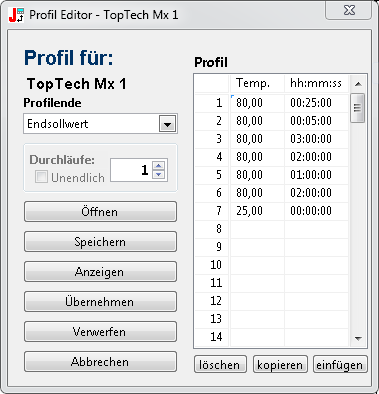
\includegraphics[width=0.5\textwidth]{img/julabo_5}
	\caption{Profileditor in \textsc{Easy Temp}}
	\label{fig:tprofil}
\end{figure}
\FloatBarrier
%Ende


\subsection{Messwertaufnahme der Temperaturprofile}
Das die aufgenommenen Messwerte der \textsc{Easy Temp}-Software nicht in der kostenfreien Variante des Programms exportiert werden können, war für die Messwertaufnahme eine externe Messung notwendig.


%Einstellungen Thermostat mit Anleitung und Support
%PC Inbetriebnahme
%Verbinden mittels COM-Stecker bzw. COM zu USB-Adapter direkt in PC
%EasyTemp gestartet und Geräte konfiguriert --> USB-Adapter funktionierte nicht --> Treiber ?
%Direkter COM-Stecker funktionierte mit Steckplatz COM1 


